\documentclass{standalone}
\usepackage{tikz}
\usepackage{hyperref}

\usetikzlibrary{shadows,calc,math,shadings}


\newcommand{\html}[2]{\href{../html/#1/explanations.html}{#2}}



\begin{document}

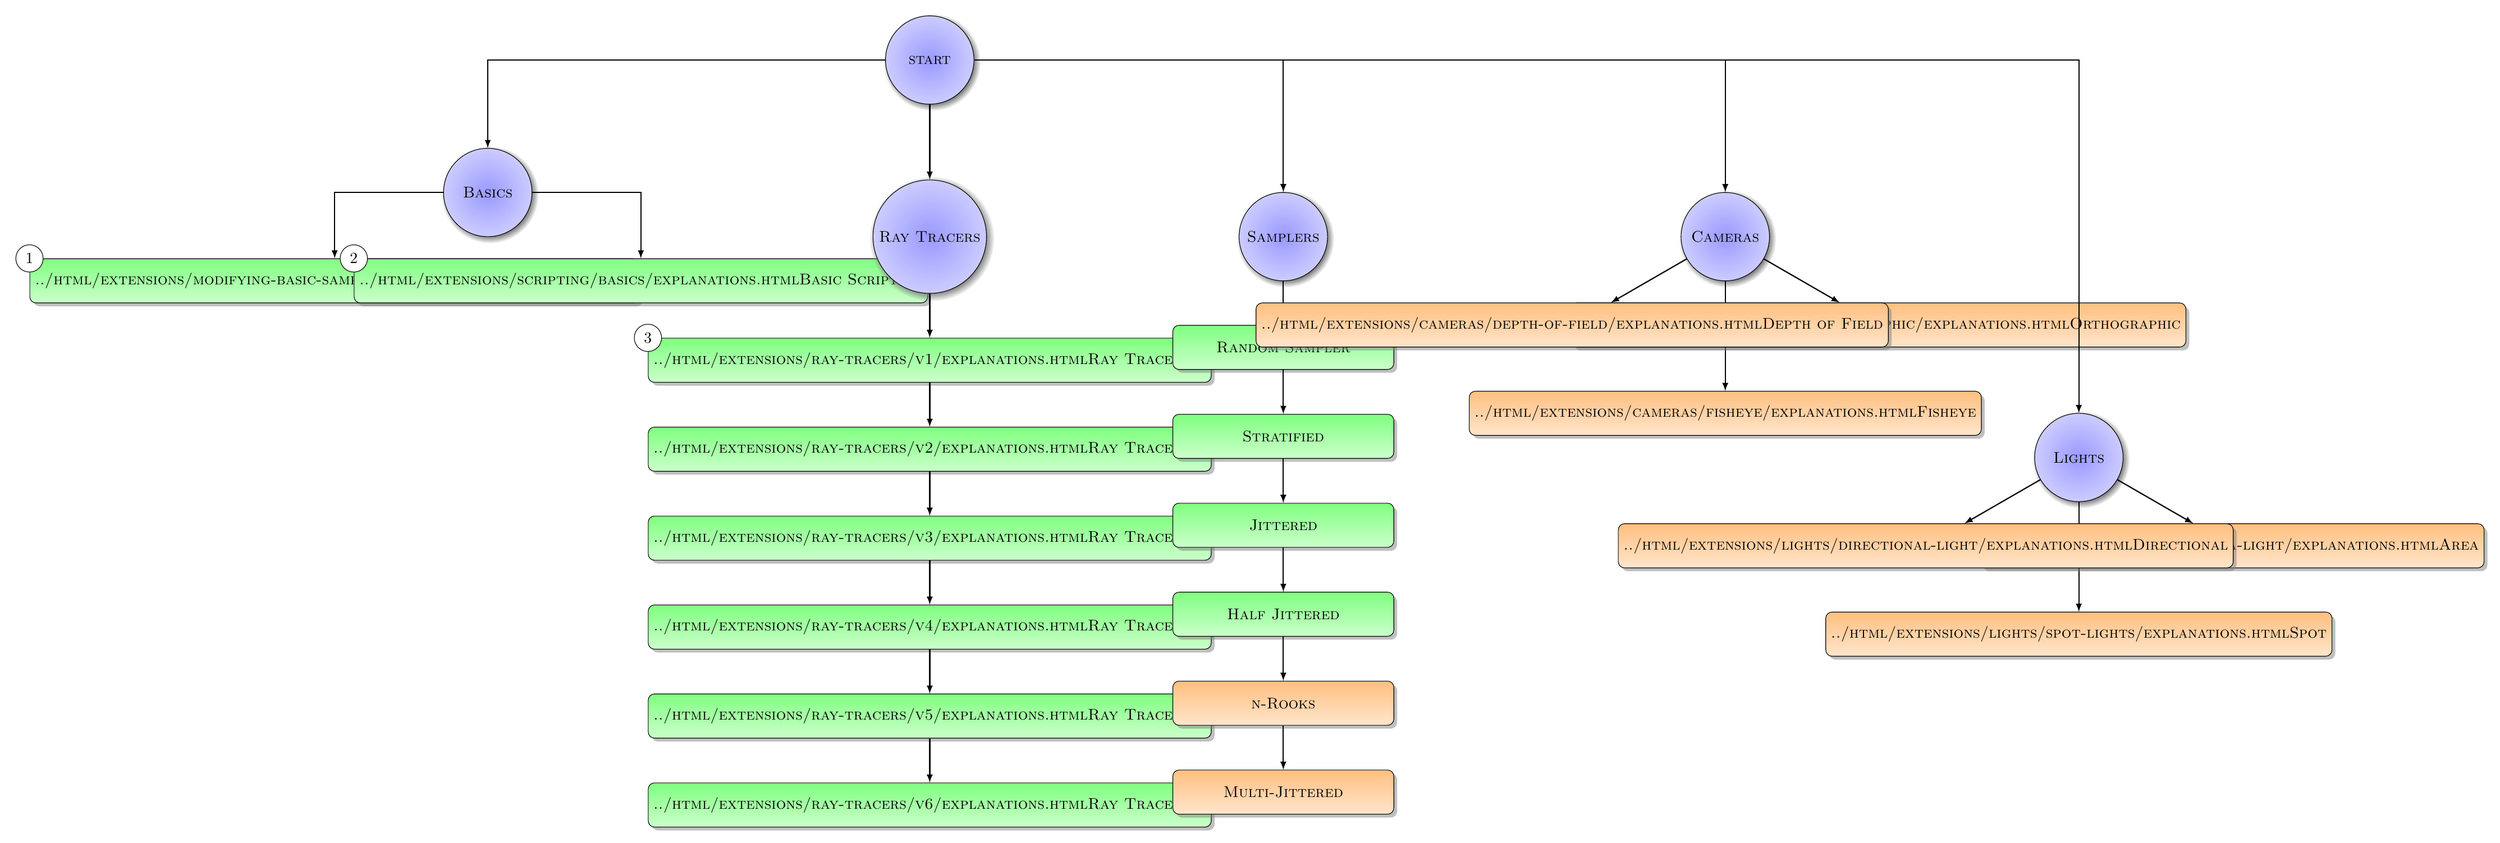
\begin{tikzpicture}[extension/.style={draw,minimum width=5cm,minimum height=1cm,font=\scshape,rounded corners=4pt,drop shadow},
                    dependency/.style={thick,latex-},
                    node/.style={circle,draw,shading=radial,minimum size=2cm,inner color=blue!40,outer color=blue!20,font=\scshape,circular drop shadow},
                    area/.style={left color=gray!30,right color=gray!10,rounded corners=4pt},
                    easy/.style={top color=green!50,bottom color=green!20},
                    medium/.style={top color=orange!50,bottom color=orange!20},
                    hard/.style={top color=red!50,bottom color=red!20},
                    order/.style={draw,circle,fill=white}]
  \pgfdeclarelayer{background}
  \pgfdeclarelayer{foreground}
  \pgfsetlayers{background,main,foreground}

  \begin{pgfonlayer}{main}
    \node[node] (start) {start};

    \node[node] (basics) at ($ (start) + (-10, -3) $) {Basics};
    \draw[dependency] (basics) |- (start);

    \node[extension,easy] (modifying basic sample) at ($ (basics) + (-150:4) $) {\html{extensions/modifying-basic-sample}{Basic Sample}};
    \draw[dependency] (modifying basic sample) |- (basics);

    \node[extension,easy] (scripting basics) at ($ (basics) + (-30:4) $) {\html{extensions/scripting/basics}{Basic Scripting}};
    \draw[dependency] (scripting basics) |- (basics);

    \node[node] (ray tracers) at ($ (start) + (0,-4) $) {Ray Tracers};
    \draw[dependency] (ray tracers) -- (start);

    \node[extension,anchor=north,easy] (ray tracer v1) at ($ (ray tracers.south) + (0,-1) $) {\html{extensions/ray-tracers/v1}{Ray Tracer v1}};
    \draw[dependency] (ray tracer v1) -- (ray tracers);

    \node[extension,anchor=north,easy] (ray tracer v2) at ($ (ray tracer v1.south) + (0,-1) $) {\html{extensions/ray-tracers/v2}{Ray Tracer v2}};
    \draw[dependency] (ray tracer v2) -- (ray tracer v1);

    \node[extension,anchor=north,easy] (ray tracer v3) at ($ (ray tracer v2.south) + (0,-1) $) {\html{extensions/ray-tracers/v3}{Ray Tracer v3}};
    \draw[dependency] (ray tracer v3) -- (ray tracer v2);

    \node[extension,anchor=north,easy] (ray tracer v4) at ($ (ray tracer v3.south) + (0,-1) $) {\html{extensions/ray-tracers/v4}{Ray Tracer v4}};
    \draw[dependency] (ray tracer v4) -- (ray tracer v3);

    \node[extension,anchor=north,easy] (ray tracer v5) at ($ (ray tracer v4.south) + (0,-1) $) {\html{extensions/ray-tracers/v5}{Ray Tracer v5}};
    \draw[dependency] (ray tracer v5) -- (ray tracer v4);

    \node[extension,anchor=north,easy] (ray tracer v6) at ($ (ray tracer v5.south) + (0,-1) $) {\html{extensions/ray-tracers/v6}{Ray Tracer v6}};
    \draw[dependency] (ray tracer v6) -- (ray tracer v5);

    \node[node] (samplers) at ($ (ray tracers) + (8,0) $) {Samplers};
    \draw[dependency] (samplers) |- (start);

    \node[extension,anchor=north,easy] (random sampler) at ($ (samplers) + (0,-2) $) {Random Sampler};
    \draw[dependency] (random sampler) -- (samplers);

    \node[extension,anchor=north,easy] (stratified sampler) at ($ (random sampler.south) + (0,-1) $) {Stratified};
    \draw[dependency] (stratified sampler) -- (random sampler);

    \node[extension,anchor=north,easy] (jittered sampler) at ($ (stratified sampler.south) + (0,-1) $) {Jittered};
    \draw[dependency] (jittered sampler) -- (stratified sampler);

    \node[extension,anchor=north,easy] (half jittered sampler) at ($ (jittered sampler.south) + (0,-1) $) {Half Jittered};
    \draw[dependency] (half jittered sampler) -- (jittered sampler);

    \node[extension,anchor=north,medium] (nrooks sampler) at ($ (half jittered sampler.south) + (0,-1) $) {n-Rooks};
    \draw[dependency] (nrooks sampler) -- (half jittered sampler);

    \node[extension,anchor=north,medium] (multijittered sampler) at ($ (nrooks sampler.south) + (0,-1) $) {Multi-Jittered};
    \draw[dependency] (multijittered sampler) -- (nrooks sampler);

    \node[node] (cameras) at ($ (samplers) + (10,0) $) {Cameras};
    \draw[dependency] (cameras) |- (start);

    \node[extension,medium] (orthographic camera) at ($ (cameras) + (-30:4) $) {\html{extensions/cameras/orthographic}{Orthographic}};
    \draw[dependency] (orthographic camera) -- (cameras);

    \node[extension,medium] (fisheye camera) at ($ (cameras) + (-90:4) $) {\html{extensions/cameras/fisheye}{Fisheye}};
    \draw[dependency] (fisheye camera) -- (cameras);

    \node[extension,medium] (depth of field camera) at ($ (cameras) + (-150:4) $) {\html{extensions/cameras/depth-of-field}{Depth of Field}};
    \draw[dependency] (depth of field camera) -- (cameras);

    \node[node] (lights) at ($ (cameras) + (8,-5) $) {Lights};
    \draw[dependency] (lights) |- (start);

    \node[extension,medium] (area light) at ($ (lights) + (-30:4) $) {\html{extensions/lights/area-light}{Area}};
    \draw[dependency] (area light) -- (lights);

    \node[extension,medium] (spot light) at ($ (lights) + (-90:4) $) {\html{extensions/lights/spot-lights}{Spot}};
    \draw[dependency] (spot light) -- (lights);

    \node[extension,medium] (directional light) at ($ (lights) + (-150:4) $) {\html{extensions/lights/directional-light}{Directional}};
    \draw[dependency] (directional light) -- (lights);
  \end{pgfonlayer}

  % \begin{pgfonlayer}{background}
  %   \draw[area] ($ (ray tracer v1.north west) + (-0.5,0.5) $) rectangle ($ (ray tracer v6.south east) + (0.5,-0.5) $);
  %   \draw[area] ($ ( random sampler.north west) + (-0.5,0.5) $) rectangle ($ (multijittered sampler.south east) + (0.5,-0.5) $);
  % \end{pgfonlayer}

  \begin{pgfonlayer}{foreground}
    \foreach[count=\i] \id in {modifying basic sample,scripting basics,ray tracer v1} {
      \node[order] at (\id.north west) {\i};
    }
  \end{pgfonlayer}
\end{tikzpicture}

\end{document}